\section{Research \& development}
This department of AllSpark is involved in all the activities related to
improve and realize new products as research projects. This sector is
considered a relevant one in the organization business, in fact this sector
has the aim to bring innovation and distinguish our products among the
competitors.

An important feature of this area is the strong collaboration between
AllSpark and various foundation operating in the OpenSource community
environment.
These collaborations are based on active support of AllSpark during the
development of their project. The support AllSpark is offering id mainly
focused on patching and bugfixing, but can be expanded to founding or other
ways of collaboration.

\subsection{Search Sector}
The main aim of this process is to look for a research sector in which
instantiate a new r\&d project. Mainly is devolved to handle security
related sectors, due to the high risks and frequent changes always present
in this area.

The process involves an analysis of the newest studies on security issues
and menaces in IT systems, its results are useful for performing an
investigation about possible vulnerabilities in AllSparks products. Is
important to notice that other than check a single product is important to
consider the whole offer of AllSpark, looking for possible problems which
are not covered by the existing products but still in the scope of AllSpark
activity.

Image \ref{2img:sector} describes this process in its details.

\begin{figure}
\begin{centering}
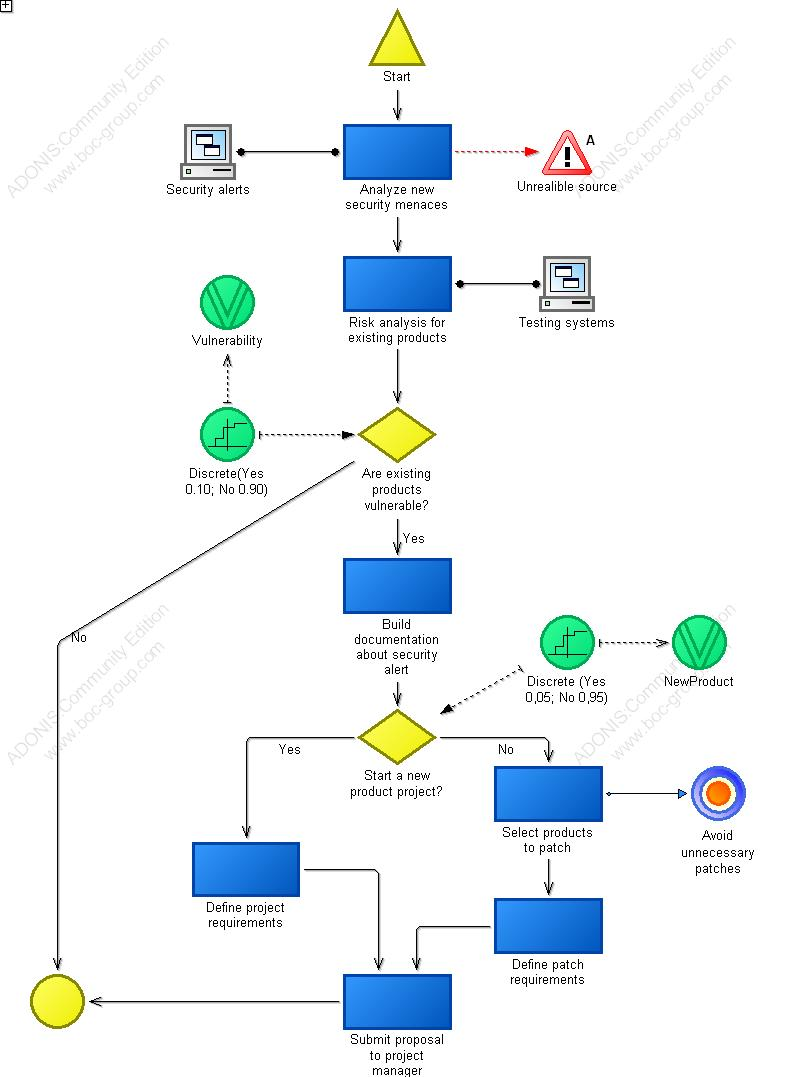
\includegraphics[scale=0.50]{assign2/adonis/imgs/sector.jpg}
\caption{Search sector AllSpark process}
\label{2img:sector}
\end{centering}
\end{figure}


\subsection{Search Updates}
In the IT environment trends and actual needs are often changing, is
therefore necessary to track these development in order to be prepared and
offer always updated products which can actually encounter costumer's
needs.

The aim of this process is to analyze the evolving market data and monitor
the trends in products usage. In this way AllSpark can retrieve a reliable
picture of the market trends.
The results of this analysis can be used to check whether there is the need
for developing a new product, or if is sufficient to add new features and
extensions to an existing one. 
